\chapter{Caminhos mínimos}

\index{caminho mínimo}

Encontrar um caminho mínimo entre dois nós
de um grafo
é um problema importante que possui muitas
aplicações práticas.
Por exemplo, um problema natural relacionado a uma rede rodoviária
é calcular o menor comprimento possível de uma rota
entre duas cidades, dados os comprimentos das estradas.

Em um grafo não ponderado, o comprimento de um caminho é igual
ao número de suas arestas, e podemos
simplesmente usar a busca em largura para encontrar
um caminho mínimo.
No entanto, neste capítulo, vamos nos concentrar em
grafos ponderados,
onde algoritmos mais sofisticados
são necessários
para encontrar caminhos mínimos.

\section{Algoritmo de Bellman–Ford}

\index{Algoritmo de Bellman–Ford}

O \key{algoritmo de Bellman–Ford}\footnote{O algoritmo recebeu o nome de
R. E. Bellman e L. R. Ford, que o publicaram independentemente
em 1958 e 1956, respectivamente \cite{bel58,for56a}.} encontra
caminhos mínimos de um nó inicial até todos os
nós do grafo.
O algoritmo pode processar todos os tipos de grafos,
desde que o grafo não contenha um
ciclo com comprimento negativo.
Se o grafo contiver um ciclo negativo,
o algoritmo pode detectar isso.

O algoritmo mantém o controle das distâncias
do nó inicial até todos os nós do grafo.
Inicialmente, a distância até o nó inicial é 0
e a distância até todos os outros nós é infinita.
O algoritmo reduz as distâncias encontrando
arestas que encurtam os caminhos até que não seja
possível reduzir nenhuma distância.

\subsubsection{Exemplo}

Vamos considerar como o algoritmo de Bellman–Ford
funciona no seguinte grafo:
\begin{center}
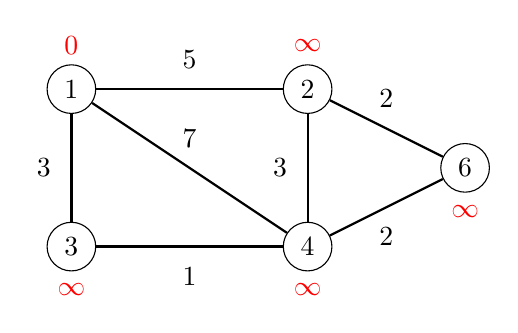
\begin{tikzpicture}
\node[draw, circle] (1) at (1,3) {1};
\node[draw, circle] (2) at (4,3) {2};
\node[draw, circle] (3) at (1,1) {3};
\node[draw, circle] (4) at (4,1) {4};
\node[draw, circle] (5) at (6,2) {6};
\node[color=red] at (1,3+0.55) {$0$};
\node[color=red] at (4,3+0.55) {$\infty$};
\node[color=red] at (1,1-0.55) {$\infty$};
\node[color=red] at (4,1-0.55) {$\infty$};
\node[color=red] at (6,2-0.55) {$\infty$};
\path[draw,thick,-] (1) -- node[font=\small,label=above:5] {} (2);
\path[draw,thick,-] (1) -- node[font=\small,label=left:3] {} (3);
\path[draw,thick,-] (3) -- node[font=\small,label=below:1] {} (4);
\path[draw,thick,-] (2) -- node[font=\small,label=left:3] {} (4);
\path[draw,thick,-] (2) -- node[font=\small,label=above:2] {} (5);
\path[draw,thick,-] (4) -- node[font=\small,label=below:2] {} (5);
\path[draw,thick,-] (1) -- node[font=\small,label=above:7] {} (4);
\end{tikzpicture}
\end{center}
Cada nó do grafo recebe uma distância.
Inicialmente, a distância até o nó inicial é 0,
e a distância até todos os outros nós é infinita.

O algoritmo procura por arestas que reduzam as distâncias.
Primeiro, todas as arestas do nó 1 reduzem as distâncias:
\begin{center}
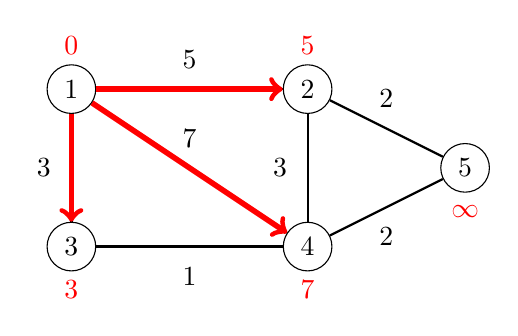
\begin{tikzpicture}
\node[draw, circle] (1) at (1,3) {1};
\node[draw, circle] (2) at (4,3) {2};
\node[draw, circle] (3) at (1,1) {3};
\node[draw, circle] (4) at (4,1) {4};
\node[draw, circle] (5) at (6,2) {5};
\node[color=red] at (1,3+0.55) {$0$};
\node[color=red] at (4,3+0.55) {$5$};
\node[color=red] at (1,1-0.55) {$3$};
\node[color=red] at (4,1-0.55) {$7$};
\node[color=red] at (6,2-0.55) {$\infty$};
\path[draw,thick,-] (1) -- node[font=\small,label=above:5] {} (2);
\path[draw,thick,-] (1) -- node[font=\small,label=left:3] {} (3);
\path[draw,thick,-] (3) -- node[font=\small,label=below:1] {} (4);
\path[draw,thick,-] (2) -- node[font=\small,label=left:3] {} (4);
\path[draw,thick,-] (2) -- node[font=\small,label=above:2] {} (5);
\path[draw,thick,-] (4) -- node[font=\small,label=below:2] {} (5);
\path[draw,thick,-] (1) -- node[font=\small,label=above:7] {} (4);

\path[draw=red,thick,->,line width=2pt] (1) -- (2);
\path[draw=red,thick,->,line width=2pt] (1) -- (3);
\path[draw=red,thick,->,line width=2pt] (1) -- (4);
\end{tikzpicture}
\end{center}
Depois disso, as arestas
$2 \rightarrow 5$ e $3 \rightarrow 4$
reduzem as distâncias:
\begin{center}
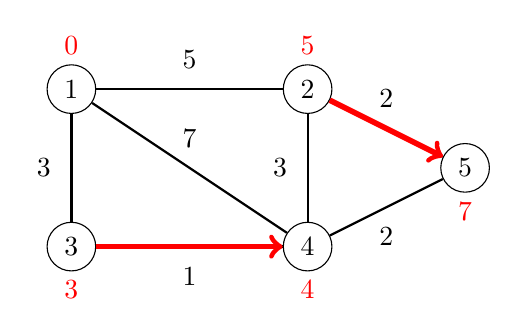
\begin{tikzpicture}
\node[draw, circle] (1) at (1,3) {1};
\node[draw, circle] (2) at (4,3) {2};
\node[draw, circle] (3) at (1,1) {3};
\node[draw, circle] (4) at (4,1) {4};
\node[draw, circle] (5) at (6,2) {5};
\node[color=red] at (1,3+0.55) {$0$};
\node[color=red] at (4,3+0.55) {$5$};
\node[color=red] at (1,1-0.55) {$3$};
\node[color=red] at (4,1-0.55) {$4$};
\node[color=red] at (6,2-0.55) {$7$};
\path[draw,thick,-] (1) -- node[font=\small,label=above:5] {} (2);
\path[draw,thick,-] (1) -- node[font=\small,label=left:3] {} (3);
\path[draw,thick,-] (3) -- node[font=\small,label=below:1] {} (4);
\path[draw,thick,-] (2) -- node[font=\small,label=left:3] {} (4);
\path[draw,thick,-] (2) -- node[font=\small,label=above:2] {} (5);
\path[draw,thick,-] (4) -- node[font=\small,label=below:2] {} (5);
\path[draw,thick,-] (1) -- node[font=\small,label=above:7] {} (4);

\path[draw=red,thick,->,line width=2pt] (2) -- (5);
\path[draw=red,thick,->,line width=2pt] (3) -- (4);
\end{tikzpicture}
\end{center}
Finalmente, há mais uma mudança:
\begin{center}
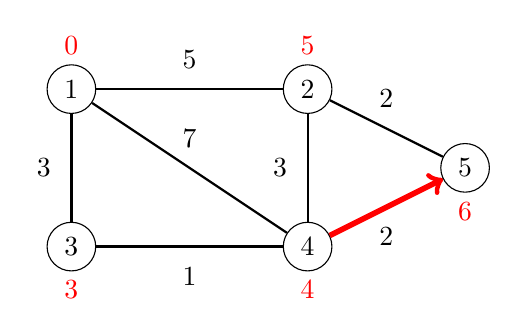
\begin{tikzpicture}
\node[draw, circle] (1) at (1,3) {1};
\node[draw, circle] (2) at (4,3) {2};
\node[draw, circle] (3) at (1,1) {3};
\node[draw, circle] (4) at (4,1) {4};
\node[draw, circle] (5) at (6,2) {5};
\node[color=red] at (1,3+0.55) {$0$};
\node[color=red] at (4,3+0.55) {$5$};
\node[color=red] at (1,1-0.55) {$3$};
\node[color=red] at (4,1-0.55) {$4$};
\node[color=red] at (6,2-0.55) {$6$};
\path[draw,thick,-] (1) -- node[font=\small,label=above:5] {} (2);
\path[draw,thick,-] (1) -- node[font=\small,label=left:3] {} (3);
\path[draw,thick,-] (3) -- node[font=\small,label=below:1] {} (4);
\path[draw,thick,-] (2) -- node[font=\small,label=left:3] {} (4);
\path[draw,thick,-] (2) -- node[font=\small,label=above:2] {} (5);
\path[draw,thick,-] (4) -- node[font=\small,label=below:2] {} (5);
\path[draw,thick,-] (1) -- node[font=\small,label=above:7] {} (4);

\path[draw=red,thick,->,line width=2pt] (4) -- (5);
\end{tikzpicture}
\end{center}

Depois disso, nenhuma aresta pode reduzir nenhuma distância.
Isso significa que as distâncias são finais,
e calculamos com sucesso
as menores distâncias
do nó inicial até todos os nós do grafo.

Por exemplo, a menor distância 3
do nó 1 ao nó 5 corresponde
ao seguinte caminho:

\begin{center}
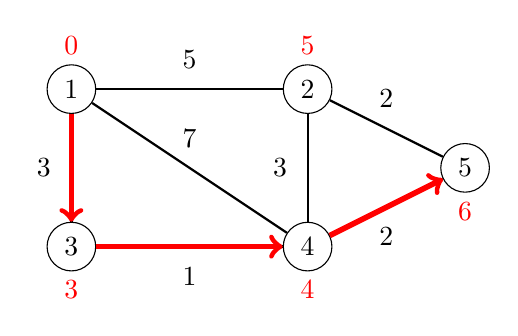
\begin{tikzpicture}
\node[draw, circle] (1) at (1,3) {1};
\node[draw, circle] (2) at (4,3) {2};
\node[draw, circle] (3) at (1,1) {3};
\node[draw, circle] (4) at (4,1) {4};
\node[draw, circle] (5) at (6,2) {5};
\node[color=red] at (1,3+0.55) {$0$};
\node[color=red] at (4,3+0.55) {$5$};
\node[color=red] at (1,1-0.55) {$3$};
\node[color=red] at (4,1-0.55) {$4$};
\node[color=red] at (6,2-0.55) {$6$};
\path[draw,thick,-] (1) -- node[font=\small,label=above:5] {} (2);
\path[draw,thick,-] (1) -- node[font=\small,label=left:3] {} (3);
\path[draw,thick,-] (3) -- node[font=\small,label=below:1] {} (4);
\path[draw,thick,-] (2) -- node[font=\small,label=left:3] {} (4);
\path[draw,thick,-] (2) -- node[font=\small,label=above:2] {} (5);
\path[draw,thick,-] (4) -- node[font=\small,label=below:2] {} (5);
\path[draw,thick,-] (1) -- node[font=\small,label=above:7] {} (4);

\path[draw=red,thick,->,line width=2pt] (1) -- (3);
\path[draw=red,thick,->,line width=2pt] (3) -- (4);
\path[draw=red,thick,->,line width=2pt] (4) -- (5);
\end{tikzpicture}
\end{center}

\subsubsection{Implementação}

A seguinte implementação do
algoritmo de Bellman–Ford determina as menores distâncias
de um nó $x$ até todos os nós do grafo.
O código assume que o grafo é armazenado
como uma lista de arestas \texttt{edges}
que consiste em tuplas da forma $(a,b,w)$,
significando que há uma aresta do nó $a$ ao nó $b$
com peso $w$.

O algoritmo consiste em $n-1$ rodadas,
e em cada rodada o algoritmo percorre
todas as arestas do grafo e tenta
reduzir as distâncias.
O algoritmo constrói um vetor \texttt{distance}
que conterá as distâncias de $x$
até todos os nós do grafo.
A constante \texttt{INF} denota uma distância infinita.

\begin{lstlisting}
for (int i = 1; i <= n; i++) distance[i] = INF;
distance[x] = 0;
for (int i = 1; i <= n-1; i++) {
    for (auto e : edges) {
        int a, b, w;
        tie(a, b, w) = e;
        distance[b] = min(distance[b], distance[a]+w);
    }
}
\end{lstlisting}

A complexidade de tempo do algoritmo é $O(nm)$,
pois o algoritmo consiste em $n-1$ rodadas e
itera por todas as $m$ arestas durante uma rodada.
Se não houver ciclos negativos no grafo,
todas as distâncias serão finais após $n-1$ rodadas,
pois cada caminho mínimo pode conter no máximo $n-1$ arestas.

Na prática, as distâncias finais geralmente podem
ser encontradas mais rapidamente do que em $n-1$ rodadas.
Assim, uma maneira possível de tornar o algoritmo mais eficiente
é pará-lo se nenhuma distância
puder ser reduzida durante uma rodada.

\subsubsection{Ciclos negativos}

\index{ciclo negativo}

O algoritmo de Bellman–Ford também pode ser usado para
verificar se o grafo contém um ciclo com comprimento negativo.
Por exemplo, o grafo

\begin{center}
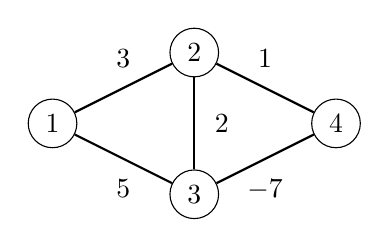
\begin{tikzpicture}[scale=0.9]
\node[draw, circle] (1) at (0,0) {$1$};
\node[draw, circle] (2) at (2,1) {$2$};
\node[draw, circle] (3) at (2,-1) {$3$};
\node[draw, circle] (4) at (4,0) {$4$};

\path[draw,thick,-] (1) -- node[font=\small,label=above:$3$] {} (2);
\path[draw,thick,-] (2) -- node[font=\small,label=above:$1$] {} (4);
\path[draw,thick,-] (1) -- node[font=\small,label=below:$5$] {} (3);
\path[draw,thick,-] (3) -- node[font=\small,label=below:$-7$] {} (4);
\path[draw,thick,-] (2) -- node[font=\small,label=right:$2$] {} (3);
\end{tikzpicture}
\end{center}
\noindent
contém um ciclo negativo
$2 \rightarrow 3 \rightarrow 4 \rightarrow 2$
com comprimento $-4$.

Se o grafo contiver um ciclo negativo,
podemos encurtar infinitamente
qualquer caminho que contenha o ciclo repetindo o ciclo
repetidamente.
Assim, o conceito de um caminho mínimo
não faz sentido nesta situação.

Um ciclo negativo pode ser detectado
usando o algoritmo de Bellman–Ford
executando o algoritmo por $n$ rodadas.
Se a última rodada reduzir alguma distância,
o grafo contém um ciclo negativo.
Observe que este algoritmo pode ser usado para
pesquisar por
um ciclo negativo em todo o grafo,
independentemente do nó inicial.

\subsubsection{Algoritmo SPFA}

\index{Algoritmo SPFA}

O \key{algoritmo SPFA} (''Shortest Path Faster Algorithm'') \cite{fan94}
é uma variante do algoritmo de Bellman–Ford,
que geralmente é mais eficiente do que o algoritmo original.
O algoritmo SPFA não percorre todas as arestas em cada rodada,
mas, em vez disso, escolhe as arestas a serem examinadas
de forma mais inteligente.

O algoritmo mantém uma fila de nós que podem
ser usados para reduzir as distâncias.
Primeiro, o algoritmo adiciona o nó inicial $x$
à fila.
Então, o algoritmo sempre processa o
primeiro nó na fila, e quando uma aresta
$a \rightarrow b$ reduz uma distância,
o nó $b$ é adicionado à fila.
% 
% The following implementation uses a 
% \texttt{queue} \texttt{q}.
% In addition, an array \texttt{inqueue} indicates
% if a node is already in the queue,
% in which case the algorithm does not add
% the node to the queue again.
% 
% \begin{lstlisting}
% for (int i = 1; i <= n; i++) distance[i] = INF;
% distance[x] = 0;
% q.push(x);
% while (!q.empty()) {
%     int a = q.front(); q.pop();
%     inqueue[a] = false;
%     for (auto b : v[a]) {
%         if (distance[a]+b.second < distance[b.first]) {
%             distance[b.first] = distance[a]+b.second;
%             if (!inqueue[b]) {q.push(b); inqueue[b] = true;}
%         }
%     }
% }
% \end{lstlisting}

A eficiência do algoritmo SPFA depende
da estrutura do grafo:
o algoritmo costuma ser eficiente,
mas sua complexidade de tempo no pior caso ainda é
$O(nm)$ e é possível criar entradas
que tornam o algoritmo tão lento quanto o
algoritmo de Bellman–Ford original.

\section{Algoritmo de Dijkstra}

\index{Algoritmo de Dijkstra}

O \key{algoritmo de Dijkstra}\footnote{E. W. Dijkstra publicou o algoritmo em 1959 \cite{dij59};
no entanto, seu artigo original não menciona como implementar o algoritmo de forma eficiente.}
encontra os caminhos mínimos
do nó inicial até todos os nós do grafo,
assim como o algoritmo de Bellman–Ford.
O benefício do algoritmo de Dijkstra é que
ele é mais eficiente e pode ser usado para
processar grafos grandes.
No entanto, o algoritmo requer que não
haja arestas com peso negativo no grafo.

Assim como o algoritmo de Bellman–Ford,
o algoritmo de Dijkstra mantém distâncias
para os nós e as reduz durante a pesquisa.
O algoritmo de Dijkstra é eficiente porque
ele só processa
cada aresta do grafo uma vez, usando o fato
de que não há arestas negativas.

\subsubsection{Exemplo}

Vamos considerar como o algoritmo de Dijkstra
funciona no seguinte grafo quando o
nó inicial é o nó 1:
\begin{center}
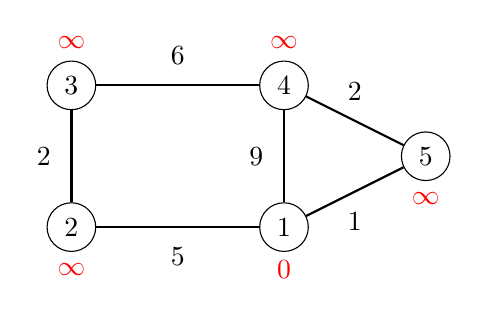
\begin{tikzpicture}[scale=0.9]
\node[draw, circle] (1) at (1,3) {3};
\node[draw, circle] (2) at (4,3) {4};
\node[draw, circle] (3) at (1,1) {2};
\node[draw, circle] (4) at (4,1) {1};
\node[draw, circle] (5) at (6,2) {5};

\node[color=red] at (1,3+0.6) {$\infty$};
\node[color=red] at (4,3+0.6) {$\infty$};
\node[color=red] at (1,1-0.6) {$\infty$};
\node[color=red] at (4,1-0.6) {$0$};
\node[color=red] at (6,2-0.6) {$\infty$};

\path[draw,thick,-] (1) -- node[font=\small,label=above:6] {} (2);
\path[draw,thick,-] (1) -- node[font=\small,label=left:2] {} (3);
\path[draw,thick,-] (3) -- node[font=\small,label=below:5] {} (4);
\path[draw,thick,-] (2) -- node[font=\small,label=left:9] {} (4);
\path[draw,thick,-] (2) -- node[font=\small,label=above:2] {} (5);
\path[draw,thick,-] (4) -- node[font=\small,label=below:1] {} (5);
\end{tikzpicture}
\end{center}
Assim como no algoritmo de Bellman–Ford,
inicialmente a distância até o nó inicial é 0
e a distância até todos os outros nós é infinita.

A cada etapa, o algoritmo de Dijkstra seleciona um nó
que ainda não foi processado e cuja distância
é a menor possível.
O primeiro nó é o nó 1 com distância 0.

Quando um nó é selecionado, o algoritmo
percorre todas as arestas que começam nesse nó
e reduz as distâncias usando-as:
\begin{center}
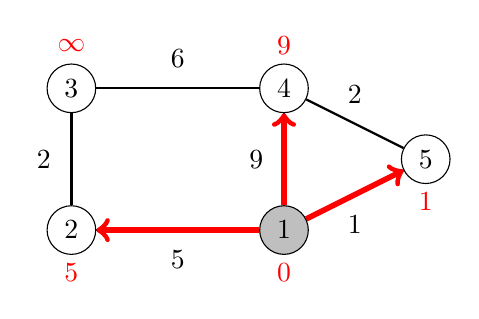
\begin{tikzpicture}[scale=0.9]
\node[draw, circle] (1) at (1,3) {3};
\node[draw, circle] (2) at (4,3) {4};
\node[draw, circle] (3) at (1,1) {2};
\node[draw, circle, fill=lightgray] (4) at (4,1) {1};
\node[draw, circle] (5) at (6,2) {5};

\node[color=red] at (1,3+0.6) {$\infty$};
\node[color=red] at (4,3+0.6) {$9$};
\node[color=red] at (1,1-0.6) {$5$};
\node[color=red] at (4,1-0.6) {$0$};
\node[color=red] at (6,2-0.6) {$1$};

\path[draw,thick,-] (1) -- node[font=\small,label=above:6] {} (2);
\path[draw,thick,-] (1) -- node[font=\small,label=left:2] {} (3);
\path[draw,thick,-] (3) -- node[font=\small,label=below:5] {} (4);
\path[draw,thick,-] (2) -- node[font=\small,label=left:9] {} (4);
\path[draw,thick,-] (2) -- node[font=\small,label=above:2] {} (5);
\path[draw,thick,-] (4) -- node[font=\small,label=below:1] {} (5);

\path[draw=red,thick,->,line width=2pt] (4) -- (2);
\path[draw=red,thick,->,line width=2pt] (4) -- (3);
\path[draw=red,thick,->,line width=2pt] (4) -- (5);
\end{tikzpicture}
\end{center}
Neste caso,
as arestas do nó 1 reduziram as distâncias dos
nós 2, 4 e 5, cujas distâncias agora são 5, 9 e 1.

O próximo nó a ser processado é o nó 5 com distância 1.
Isso reduz a distância até o nó 4 de 9 para 3:
\begin{center}
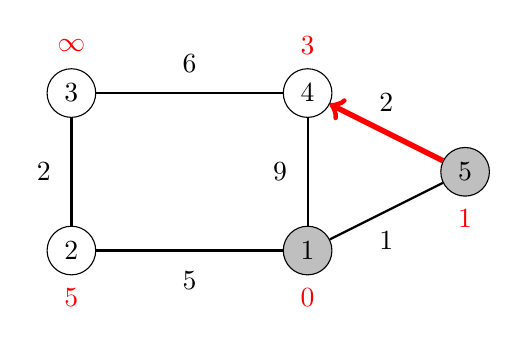
\begin{tikzpicture}
\node[draw, circle] (1) at (1,3) {3};
\node[draw, circle] (2) at (4,3) {4};
\node[draw, circle] (3) at (1,1) {2};
\node[draw, circle, fill=lightgray] (4) at (4,1) {1};
\node[draw, circle, fill=lightgray] (5) at (6,2) {5};

\node[color=red] at (1,3+0.6) {$\infty$};
\node[color=red] at (4,3+0.6) {$3$};
\node[color=red] at (1,1-0.6) {$5$};
\node[color=red] at (4,1-0.6) {$0$};
\node[color=red] at (6,2-0.6) {$1$};

\path[draw,thick,-] (1) -- node[font=\small,label=above:6] {} (2);
\path[draw,thick,-] (1) -- node[font=\small,label=left:2] {} (3);
\path[draw,thick,-] (3) -- node[font=\small,label=below:5] {} (4);
\path[draw,thick,-] (2) -- node[font=\small,label=left:9] {} (4);
\path[draw,thick,-] (2) -- node[font=\small,label=above:2] {} (5);
\path[draw,thick,-] (4) -- node[font=\small,label=below:1] {} (5);

\path[draw=red,thick,->,line width=2pt] (5) -- (2);
\end{tikzpicture}
\end{center}
Depois disso, o próximo nó é o nó 4, que reduz
a distância até o nó 3 para 9:
\begin{center}
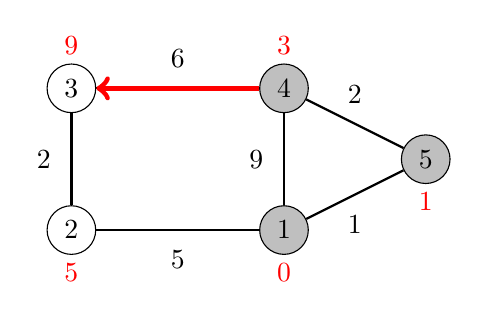
\begin{tikzpicture}[scale=0.9]
\node[draw, circle] (1) at (1,3) {3};
\node[draw, circle, fill=lightgray] (2) at (4,3) {4};
\node[draw, circle] (3) at (1,1) {2};
\node[draw, circle, fill=lightgray] (4) at (4,1) {1};
\node[draw, circle, fill=lightgray] (5) at (6,2) {5};

\node[color=red] at (1,3+0.6) {$9$};
\node[color=red] at (4,3+0.6) {$3$};
\node[color=red] at (1,1-0.6) {$5$};
\node[color=red] at (4,1-0.6) {$0$};
\node[color=red] at (6,2-0.6) {$1$};

\path[draw,thick,-] (1) -- node[font=\small,label=above:6] {} (2);
\path[draw,thick,-] (1) -- node[font=\small,label=left:2] {} (3);
\path[draw,thick,-] (3) -- node[font=\small,label=below:5] {} (4);
\path[draw,thick,-] (2) -- node[font=\small,label=left:9] {} (4);
\path[draw,thick,-] (2) -- node[font=\small,label=above:2] {} (5);
\path[draw,thick,-] (4) -- node[font=\small,label=below:1] {} (5);

\path[draw=red,thick,->,line width=2pt] (2) -- (1);
\end{tikzpicture}
\end{center}

Uma propriedade notável do algoritmo de Dijkstra é que
sempre que um nó é selecionado, sua distância é final.
Por exemplo, neste ponto do algoritmo,
as distâncias 0, 1 e 3 são as distâncias finais
até os nós 1, 5 e 4.

Depois disso, o algoritmo processa os dois
nós restantes, e as distâncias finais são as seguintes:

\begin{center}
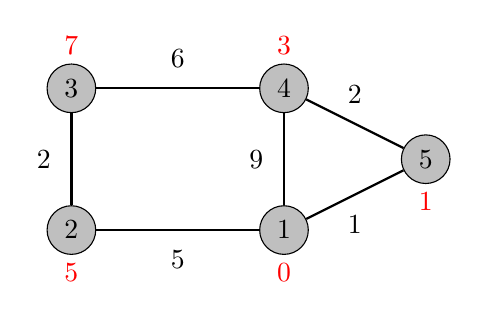
\begin{tikzpicture}[scale=0.9]
\node[draw, circle, fill=lightgray] (1) at (1,3) {3};
\node[draw, circle, fill=lightgray] (2) at (4,3) {4};
\node[draw, circle, fill=lightgray] (3) at (1,1) {2};
\node[draw, circle, fill=lightgray] (4) at (4,1) {1};
\node[draw, circle, fill=lightgray] (5) at (6,2) {5};

\node[color=red] at (1,3+0.6) {$7$};
\node[color=red] at (4,3+0.6) {$3$};
\node[color=red] at (1,1-0.6) {$5$};
\node[color=red] at (4,1-0.6) {$0$};
\node[color=red] at (6,2-0.6) {$1$};

\path[draw,thick,-] (1) -- node[font=\small,label=above:6] {} (2);
\path[draw,thick,-] (1) -- node[font=\small,label=left:2] {} (3);
\path[draw,thick,-] (3) -- node[font=\small,label=below:5] {} (4);
\path[draw,thick,-] (2) -- node[font=\small,label=left:9] {} (4);
\path[draw,thick,-] (2) -- node[font=\small,label=above:2] {} (5);
\path[draw,thick,-] (4) -- node[font=\small,label=below:1] {} (5);
\end{tikzpicture}
\end{center}

\subsubsection{Arestas negativas}

A eficiência do algoritmo de Dijkstra é
baseada no fato de que o grafo não
contém arestas negativas.
Se houver uma aresta negativa,
o algoritmo pode dar resultados incorretos.
Como exemplo, considere o seguinte grafo:

\begin{center}
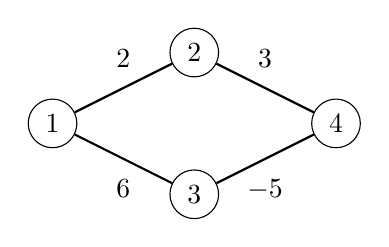
\begin{tikzpicture}[scale=0.9]
\node[draw, circle] (1) at (0,0) {$1$};
\node[draw, circle] (2) at (2,1) {$2$};
\node[draw, circle] (3) at (2,-1) {$3$};
\node[draw, circle] (4) at (4,0) {$4$};

\path[draw,thick,-] (1) -- node[font=\small,label=above:2] {} (2);
\path[draw,thick,-] (2) -- node[font=\small,label=above:3] {} (4);
\path[draw,thick,-] (1) -- node[font=\small,label=below:6] {} (3);
\path[draw,thick,-] (3) -- node[font=\small,label=below:$-5$] {} (4);
\end{tikzpicture}
\end{center}
\noindent
O caminho mínimo do nó 1 ao nó 4 é
$1 \rightarrow 3 \rightarrow 4$
e seu comprimento é 1.
No entanto, o algoritmo de Dijkstra
encontra o caminho $1 \rightarrow 2 \rightarrow 4$
seguindo as arestas de menor peso.
O algoritmo não leva em consideração que
no outro caminho, o peso $-5$
compensa o peso grande anterior $6$.

\subsubsection{Implementação}

A seguinte implementação do algoritmo de Dijkstra
calcula as distâncias mínimas de um nó $x$
para outros nós do grafo.
O grafo é armazenado como listas de adjacência
de modo que \texttt{adj[$a$]} contém um par $(b,w)$
sempre que houver uma aresta do nó $a$ ao nó $b$
com peso $w$.

Uma implementação eficiente do algoritmo de Dijkstra
exige que seja possível encontrar eficientemente o
nó de distância mínima que ainda não foi processado.
Uma estrutura de dados apropriada para isso é uma fila de prioridade
que contém os nós ordenados por suas distâncias.
Usando uma fila de prioridade, o próximo nó a ser processado
pode ser recuperado em tempo logarítmico.

No código a seguir, a fila de prioridade
\texttt{q} contém pares da forma $(-d,x)$,
o que significa que a distância atual até o nó $x$ é $d$.
O vetor $\texttt{distance}$ contém a distância até
cada nó, e o vetor $\texttt{processed}$ indica
se um nó já foi processado.
Inicialmente, a distância é $0$ para $x$ e $\infty$ para todos os outros nós.

\begin{lstlisting}
for (int i = 1; i <= n; i++) distance[i] = INF;
distance[x] = 0;
q.push({0,x});
while (!q.empty()) {
    int a = q.top().second; q.pop();
    if (processed[a]) continue;
    processed[a] = true;
    for (auto u : adj[a]) {
        int b = u.first, w = u.second;
        if (distance[a]+w < distance[b]) {
            distance[b] = distance[a]+w;
            q.push({-distance[b],b});
        }
    }
}
\end{lstlisting}

Observe que a fila de prioridade contém distâncias
\emph{negativas} até os nós.
A razão para isso é que a
versão padrão da fila de prioridade em C++ encontra elementos máximos,
enquanto queremos encontrar elementos mínimos.
Usando distâncias negativas,
podemos usar diretamente a fila de prioridade padrão\footnote{Claro,
também poderíamos declarar a fila de prioridade como no Capítulo 4.5
e usar distâncias positivas, mas a implementação seria um pouco mais longa.}.
Observe também que pode haver várias instâncias do mesmo
nó na fila de prioridade; no entanto, apenas a instância com a
distância mínima será processada.

A complexidade de tempo da implementação acima é
$O(n+m \log m)$, pois o algoritmo percorre
todos os nós do grafo e adiciona para cada aresta
no máximo uma distância à fila de prioridade.

\section{Algoritmo de Floyd–Warshall}

\index{Algoritmo de Floyd–Warshall}

O \key{algoritmo de Floyd–Warshall}\footnote{O algoritmo
recebeu o nome de R. W. Floyd e S. Warshall,
que o publicaram independentemente em 1962 \cite{flo62,war62}.}
fornece uma maneira alternativa de abordar o problema
de encontrar caminhos mínimos.
Ao contrário dos outros algoritmos deste capítulo,
ele encontra todos os caminhos mínimos entre os nós
em uma única execução.

O algoritmo mantém uma matriz bidimensional
que contém as distâncias entre os nós.
Primeiro, as distâncias são calculadas usando apenas
arestas diretas entre os nós,
e depois disso, o algoritmo reduz as distâncias
usando nós intermediários nos caminhos.

\subsubsection{Exemplo}

Vamos considerar como o algoritmo de Floyd–Warshall
funciona no seguinte grafo:

\begin{center}
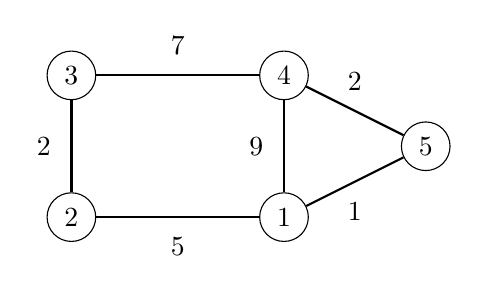
\begin{tikzpicture}[scale=0.9]
\node[draw, circle] (1) at (1,3) {$3$};
\node[draw, circle] (2) at (4,3) {$4$};
\node[draw, circle] (3) at (1,1) {$2$};
\node[draw, circle] (4) at (4,1) {$1$};
\node[draw, circle] (5) at (6,2) {$5$};

\path[draw,thick,-] (1) -- node[font=\small,label=above:7] {} (2);
\path[draw,thick,-] (1) -- node[font=\small,label=left:2] {} (3);
\path[draw,thick,-] (3) -- node[font=\small,label=below:5] {} (4);
\path[draw,thick,-] (2) -- node[font=\small,label=left:9] {} (4);
\path[draw,thick,-] (2) -- node[font=\small,label=above:2] {} (5);
\path[draw,thick,-] (4) -- node[font=\small,label=below:1] {} (5);
\end{tikzpicture}
\end{center}

Inicialmente, a distância de cada nó para si mesmo é $0$,
e a distância entre os nós $a$ e $b$ é $x$
se houver uma aresta entre os nós $a$ e $b$ com peso $x$.
Todas as outras distâncias são infinitas.

Neste grafo, a matriz inicial é a seguinte:
\begin{center}
\begin{tabular}{r|rrrrr}
 & 1 & 2 & 3 & 4 & 5 \\
\hline
1 & 0 & 5 & $\infty$ & 9 & 1 \\
2 & 5 & 0 & 2 & $\infty$ & $\infty$ \\
3 & $\infty$ & 2 & 0 & 7 & $\infty$ \\
4 & 9 & $\infty$ & 7 & 0 & 2 \\
5 & 1 & $\infty$ & $\infty$ & 2 & 0 \\
\end{tabular}
\end{center}
\vspace{10pt}
O algoritmo consiste em rodadas consecutivas.
Em cada rodada, o algoritmo seleciona um novo nó
que pode atuar como um nó intermediário nos caminhos a partir de agora,
e as distâncias são reduzidas usando este nó.

Na primeira rodada, o nó 1 é o novo nó intermediário.
Há um novo caminho entre os nós 2 e 4
com comprimento 14, pois o nó 1 os conecta.
Há também um novo caminho
entre os nós 2 e 5 com comprimento 6.

\begin{center}
\begin{tabular}{r|rrrrr}
 & 1 & 2 & 3 & 4 & 5 \\
\hline
1 & 0 & 5 & $\infty$ & 9 & 1 \\
2 & 5 & 0 & 2 & \textbf{14} & \textbf{6} \\
3 & $\infty$ & 2 & 0 & 7 & $\infty$ \\
4 & 9 & \textbf{14} & 7 & 0 & 2 \\
5 & 1 & \textbf{6} & $\infty$ & 2 & 0 \\
\end{tabular}
\end{center}
\vspace{10pt}

Na segunda rodada, o nó 2 é o novo nó intermediário.
Isso cria novos caminhos entre os nós 1 e 3
e entre os nós 3 e 5:

\begin{center}
\begin{tabular}{r|rrrrr}
 & 1 & 2 & 3 & 4 & 5 \\
\hline
1 & 0 & 5 & \textbf{7} & 9 & 1 \\
2 & 5 & 0 & 2 & 14 & 6 \\
3 & \textbf{7} & 2 & 0 & 7 & \textbf{8} \\
4 & 9 & 14 & 7 & 0 & 2 \\
5 & 1 & 6 & \textbf{8} & 2 & 0 \\
\end{tabular}
\end{center}
\vspace{10pt}

Na terceira rodada, o nó 3 é o novo nó intermediário.
Há um novo caminho entre os nós 2 e 4:

\begin{center}
\begin{tabular}{r|rrrrr}
 & 1 & 2 & 3 & 4 & 5 \\
\hline
1 & 0 & 5 & 7 & 9 & 1 \\
2 & 5 & 0 & 2 & \textbf{9} & 6 \\
3 & 7 & 2 & 0 & 7 & 8 \\
4 & 9 & \textbf{9} & 7 & 0 & 2 \\
5 & 1 & 6 & 8 & 2 & 0 \\
\end{tabular}
\end{center}
\vspace{10pt}

O algoritmo continua assim,
até que todos os nós tenham sido designados nós intermediários.
Depois que o algoritmo termina, a matriz contém
as distâncias mínimas entre quaisquer dois nós:

\begin{center}
\begin{tabular}{r|rrrrr}
 & 1 & 2 & 3 & 4 & 5 \\
\hline
1 & 0 & 5 & 7 & 3 & 1 \\
2 & 5 & 0 & 2 & 8 & 6 \\
3 & 7 & 2 & 0 & 7 & 8 \\
4 & 3 & 8 & 7 & 0 & 2 \\
5 & 1 & 6 & 8 & 2 & 0 \\
\end{tabular}
\end{center}

Por exemplo, a matriz nos diz que a
menor distância entre os nós 2 e 4 é 8.
Isso corresponde ao seguinte caminho:

\begin{center}
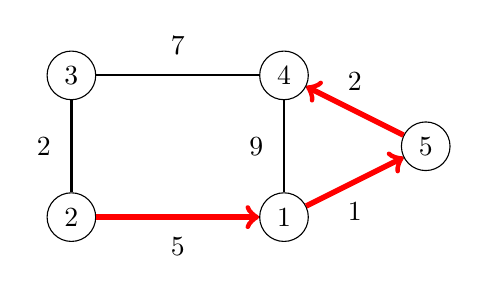
\begin{tikzpicture}[scale=0.9]
\node[draw, circle] (1) at (1,3) {$3$};
\node[draw, circle] (2) at (4,3) {$4$};
\node[draw, circle] (3) at (1,1) {$2$};
\node[draw, circle] (4) at (4,1) {$1$};
\node[draw, circle] (5) at (6,2) {$5$};

\path[draw,thick,-] (1) -- node[font=\small,label=above:7] {} (2);
\path[draw,thick,-] (1) -- node[font=\small,label=left:2] {} (3);
\path[draw,thick,-] (3) -- node[font=\small,label=below:5] {} (4);
\path[draw,thick,-] (2) -- node[font=\small,label=left:9] {} (4);
\path[draw,thick,-] (2) -- node[font=\small,label=above:2] {} (5);
\path[draw,thick,-] (4) -- node[font=\small,label=below:1] {} (5);

\path[draw=red,thick,->,line width=2pt] (3) -- (4);
\path[draw=red,thick,->,line width=2pt] (4) -- (5);
\path[draw=red,thick,->,line width=2pt] (5) -- (2);
\end{tikzpicture}
\end{center}

\subsubsection{Implementação}

A vantagem do
algoritmo de Floyd–Warshall é que ele é
fácil de implementar.
O código a seguir constrói uma
matriz de distância onde $\texttt{distance}[a][b]$
é a menor distância entre os nós $a$ e $b$.
Primeiro, o algoritmo inicializa \texttt{distance}
usando a matriz de adjacência \texttt{adj} do grafo:

\begin{lstlisting}
for (int i = 1; i <= n; i++) {
    for (int j = 1; j <= n; j++) {
        if (i == j) distance[i][j] = 0;
        else if (adj[i][j]) distance[i][j] = adj[i][j];
        else distance[i][j] = INF;
    }
}
\end{lstlisting}
Depois disso, as menores distâncias podem ser encontradas da seguinte forma:
\begin{lstlisting}
for (int k = 1; k <= n; k++) {
    for (int i = 1; i <= n; i++) {
        for (int j = 1; j <= n; j++) {
            distance[i][j] = min(distance[i][j],
                                   distance[i][k]+distance[k][j]);
        }
    }
}
\end{lstlisting}

A complexidade de tempo do algoritmo é $O(n^3)$,
pois ele contém três loops aninhados
que percorrem os nós do grafo.

Como a implementação do algoritmo de Floyd–Warshall
é simples, o algoritmo pode ser
uma boa escolha mesmo que seja necessário encontrar apenas um
único caminho mínimo no grafo.
No entanto, o algoritmo só pode ser usado quando o grafo
é tão pequeno que uma complexidade de tempo cúbica é rápida o suficiente.
